\chapter{Ковалентная и ионная связи. Молекула водорода. Адиабатическое 
приближение. Теория Гайтлера -- Лондона. Многоатомные молекулы. 
Электронные состояния. Принцип Франка-Кондона. Колебательные состояния. 
Вращательные состояния.}

\section{Ковалентная и ионная связи}
\emph{Ковалентная связь} образуется при перекрытии валентных электронных 
облаков, то есть часть электронов движется около обоих ядер одновременно.

\emph{Ионная связь:} электроны в молекуле можно разделить на две группы 
при этом каждая из групп находится возле одного из ядер. Эти группы делят 
между собой электроны так, что в одной из групп избыток, а в другой 
недостаток. В результате молекула состоит из двух ионов противоположных 
знаков притягивающихся друг к другу.

\section{Молекула водорода}
После создания квантовой механики Гайтлер и Лондон предприняли успешную 
попутку квантовомеханического расчёта основного состояния молекулы 
\( H_2 \). Им удалось решить уравнение Шрёдингера для системы, состоящей 
из двух протонов и двух электронов.

\begin{figure}[h!]
    \center
    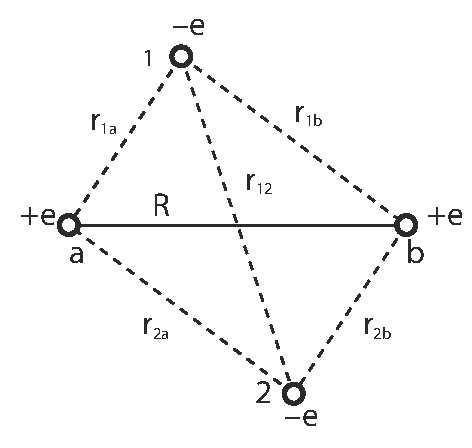
\includegraphics[width=.47\textwidth]{15_01}
\end{figure}

Потенциальная энергия такой системы равна
\[ 
	U = -\frac{e^2}{r_{1a}} - \frac{e^2}{r_{2a}} - \frac{e^2}{r_{1b}} -
	\frac{e^2}{r_{2b}} + \frac{e^2}{r_{12}} + \frac{e^2}{R} 
\]
Волновая функция \( \psi \) зависит от координат обоих электронов. 
Следовательно, уравнение Шрёдингера имеет вид:
\[ 
	\Delta_1\psi + \Delta_2\psi + \frac{2m_e}{\hbar^2}
	\left(E - e^2\left( \frac{1}{r_{12}} + \frac{1}{R} -
	\frac{1}{r_{1a}} - \frac{1}{r_{2a}} - \frac{1}{r_{1b}} -
	\frac{1}{r_{2b}}\right) \right)\psi = 0
\]
где \( \Delta_1 \) -- оператор Лапласа, содержащий координаты 
одного электрона, а \( \Delta_2 \) -- оператор Лапласа, содержащий 
координаты другого электрона.

Получающиеся из предыдущего уравнения собственные значения 
энергии оказываются зависящими от расстояния между ядрами \( R \), 
то есть \( E = E(R) \), причём в случаях параллельной и 
антипараллельной ориентации спинов характер этой зависимости существенно 
различен (рис. 15.02). Образование молекулы возможно лиши при сближении 
атомов с антипараллельными спинами.

Асимптотическое значение \( E_0 \), к которому стремится энергия 
молекулы при \( R \rightarrow \infty \), для обеих кривых одинаково 
и равно сумме энергий изолированных атомов. Величина \( E_D \) есть 
энергия связи молекулы. Она равна энергии, которую нужно сообщить 
молекуле, чтобы вызвать разделение её на изолированные атомы, то есть 
вызвать диссоциацию молекулы.

\begin{figure}[h!]
    \center
    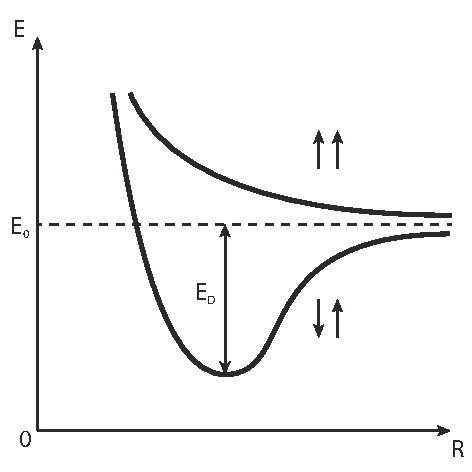
\includegraphics[width=.47\textwidth]{15_02}
\end{figure}

\section{Адиабатическое приближение}
\emph{Адиабатическое приближение} -- это метод приближения решения задач в 
квантовой механике, для описания квантовых систем, в которых можно выделить 
"быструю" и "медленную" подсистему. 

Исходная задача решается в два этапа:
\begin{enumerate}
    \item рассматриваем движение "быстрой" подсистемы при фиксированной 
        координатах "медленно" подсистемы
    \item учитываем определенным образом "медленную" подсистему
\end{enumerate}

\section{Теория Гайтлера -- Лондона}
В основе теории валентных связей лежит гипотеза о том, что при 
образовании молекулы из атомов, последние в значительной мере сохраняют 
свою электронную конфигурацию, а связывание атомов достигается в 
результате обмена электронов между ними и спаривания спинов двух 
электронов, находящихся на атомных орбиталях исходных атомов. 

\section{Многоатомные молекулы}
Спектры многоатомных молекул изучать чисто оптическими методами
довольно сложно, так как вращательные и колебательные спектры этих
молекул обычно лежат в далекой инфракрасной области. Интенсивность их
линий в спектрах испускания мала, особенно для вещества, находящегося в
газообразном состоянии.

Поэтому инфракрасные спектры в большинстве случаев наблюдаются в
виде спектров поглощения.

Согласно классической механике вращательная энергия молекулы
определяется ее моментом инерции \( J \) и квадратом угловой скорости
молекулы. Запишем выражение инерции молекулы относительно всех трёх 
осей декартовой системы координат:
\[ 
	J_{xx} = \sum_i m_i\left( y^2_i + z^2_i \right);\quad
	J_{xy} = \sum_i m_i x_i y_i
\]
\[ 
	J_{yy} = \sum_i m_i\left( x^2_i + z^2_i \right);\quad
	J_{xz} = \sum_i m_i x_i z_i
\]
\[ 
	J_{zz} = \sum_i m_i\left( x^2_i + y^2_i \right);\quad
	J_{yz} = \sum_i m_i y_i z_i
\]

Многоатомные молекулы можно разделить на несколько классов в
зависимости от вида их эллипсоидов инерции:
\begin{enumerate}
	\item Линейные молекулы (момент инерции относительно оси, 
		соединяющей все атомы молекулы, равен нулю, а два 
		других оказываются равными друг другу)
	\item Симметричный волчок (эллипсоид инерции является эллипсоидом
		вращения вокруг оси, которая является одной из его главных осей 
		и в то же время является осью волчка)
	\item Сферический волчок (если молекула обладает шарообразным
		эллипсоидом инерции, то есть если \( J_{xx} = J_{yy} = J_{zz}\), 
		то такая молекула называется молекулой типа сферического волчка)
	\item Асимметричный волчок (\( J_{xx} \neq J_{yy} \neq J_{zz} \))
\end{enumerate}

\section{Электронные состояния}
Полная энергия молекулы состоит из трёх основных составляющих:
\begin{enumerate}
	\item \( E_e \) -- электронная энергия (энергия обусловленная 
		движением электронов)
	\item \( E_v \) -- колебательная составляющая энергии (
		обусловлена колебанием ядер)
	\item \( E_r \) -- вращательная энергия (обусловлена вращением 
		молекулы в целом)
\end{enumerate}
В первом приближении можно считать, что эти все виды энергии независимы 
друг от друга \( E_e \) меняется при изменении электронной конфигурации 
молекулы. При изменении электронной энергии будут также изменяться 
\( E_v \) и  \( E_r \).

\section{Принцип Франка-Кондона}
\emph{электронный переход происходит наиболее вероятно без 
изменения положений ядер молекулы.}

\section{Колебательные состояния}
Рассмотрим гармонический осциллятор, то есть частицу находящуюся под 
действием квазиупругой силы \( F = -kx \). Потенциальная энергия 
такой частицы равна:
\[ U = \frac{kx^2}{2} \]
Введя собственную частоту \( \omega_v = \sqrt{k/m} \) классического 
гармонического осциллятора, можно написать:
\[ U = \frac{m\omega^2_v x^2}{2} \]
Следовательно, уравнение Шрёдингера для гармонического осциллятора 
выглядит следующим образом:
\[ 
	\dder{\psi}{x} + \frac{2m}{\hbar^2}
	\left( E_v - \frac{m\omega^2_v x^2}{2}\right)\psi = 0
\]
где \( E_v \) -- полная энергия осциллятора. Это уравнение имеет 
конечные, однозначные и непрерывные решения при значениях параметра 
\( E_v \), равных
\[ E_v = \left(v + \frac{1}{2}\right)\hbar\omega_v \]
Число \( v \), называемое \emph{колебательным квантовым числом}, 
может иметь значения: \( 0, 1, 2 \) и т.д.
Для колебательного квантового числа \( v \) имеется правило отбора:
\[ \Delta v = \pm 1 \]
Поэтому энергия гармонического осциллятора может изменяться только 
порциями \( \hbar\omega_v \)

\section{Вращательные состояния}
Энергия системы, имеющей момент инерции \( I \) и вращающейся с 
угловой скоростью \( \omega_r \), равна 
\[ 
	E_r = \frac{I\omega^2_r}{2} = \frac{(I\omega_r)^2}{2I} = 
	\frac{M^2}{2I}
\]
где \( M = I\omega_r \) -- момент импульса системы. Согласно 
квантовой механике момент импульса может принимать лишь 
дискретные значения:
\[ M = \hbar\sqrt{J(J+1)} \]
Следовательно, вращательная энергия молекулы может иметь только 
квантованные значения:
\[ E_r = \frac{\hbar^2}{2I}J(J+1) \]
где \( I \) -- момент инерции молекулы относительно оси, проходящей 
через её центр инерции, \( J \) -- вращательное квантовое число.

\newpage
